\subsection{External Wishbone Slave/Master interface}
\label{sec:wrpc_wb}

%\begin{figure}[ht]
%  \begin{center}
%    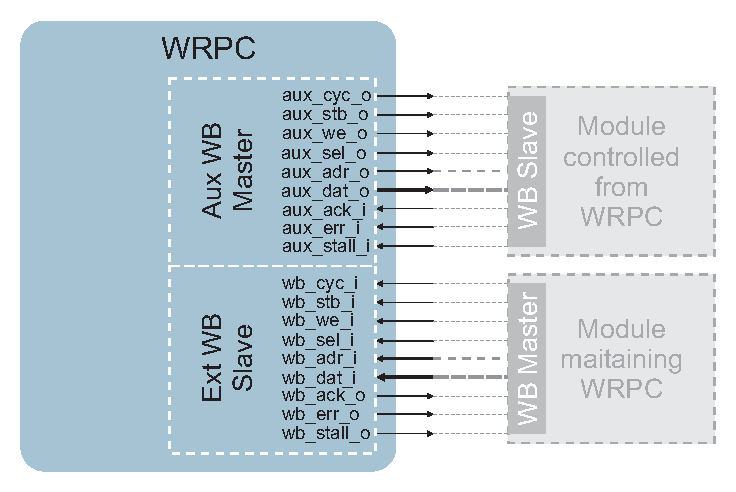
\includegraphics[width=.7\textwidth]{fig/wrpc_wb.pdf}
%    \caption{External Wishbone interfaces of WRPC}
%  \end{center}
%\end{figure}

{\bf Ext WB Slave} is a Wishbone slave interface (see the Wishbone bus specification~\cite{wb_spec}
for more details). It controls the primary Wishbone Crossbar insisde the WRPC and thus provides
access to all the WRPC internals.

In most designs, this slave interface should be connected to the host (if any), via an aprropriate
bridge. As an example, in the SPEC WRPC reference design it is connected to a Gennum GN4124 IP core,
and in the SVEC/VFC-HD reference designs it is connected to the VME64x IP core.  In all three
reference designs, this interface is used to upload WRPC software to its internal memory and to
access the WRPC VUART.

HDL modules accessible through \emph{Ext WB Slave} interface include:
\begin{center}
  \begin{tabular}{|l|l|}
    \hline {\bf module name} & {\bf offset (bytes)}\\
    \hline
    WRPC internal memory & 0x00000\\
                Mini NIC & 0x20000\\
                Endpoint & 0x20100\\
                Soft PLL & 0x20200\\
           PPS generator & 0x20300\\
                  Syscon & 0x20400\\
                    UART & 0x20500\\
           1-Wire Master & 0x20600\\
           Aux WB Master & 0x20700\\
    \hline
  \end{tabular}
\end{center}

{\bf Aux WB Master} is a Pipelined Wishbone Master interface. It is connected through the Wishbone
Crossbar inside the White Rabbit PTP Core to the LM32 soft-core processor (instantiated inside the
WRPC). It can optionally be used to control any user-defined module having a Pipelined Wishbone
Slave interface. In that case, the WRPC software has to be modified to control additional modules
connected to the \emph{Aux WB Master} interface. An alternative is to access the Aux WB master
interface from the host (via the external Wishbone slave interface).

